\documentclass{article}
\usepackage{tikz}
\usetikzlibrary{arrows.meta,shapes.misc,decorations.pathmorphing,calc}
\usetikzlibrary{fit, positioning, backgrounds}

\begin{document}
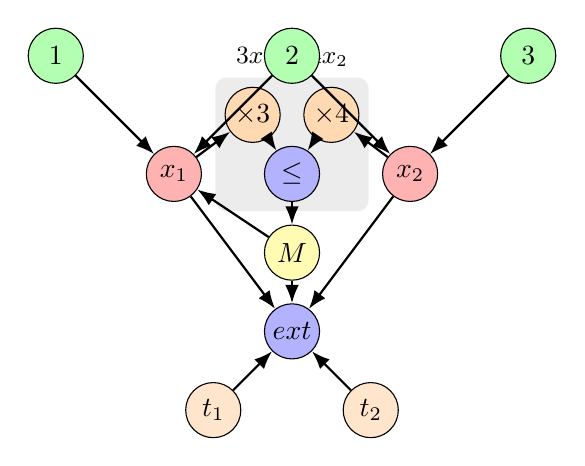
\begin{tikzpicture}[
    % Styles
    vertex/.style={circle, draw, minimum size=7mm, inner sep=0pt},
    edge/.style={draw, thick, -{Latex}},
    values/.style={vertex, fill=green!30},
    variables/.style={vertex, fill=red!30},
    constraints/.style={vertex, fill=blue!30},
    operators/.style={vertex, fill=orange!30},
    model/.style={vertex, fill=yellow!30},
    tuples/.style={vertex, fill=orange!20},
    highlight/.style={rectangle, rounded corners, fill=gray!30, opacity=0.5},
    % Margins
    margin/.style={solid, one side expanded=1mm}
  ]

  %% Vertices
  % Values
  \node[values] (v1) at (0, 3) {1};
  \node[values] (v2) at (3, 3) {2};
  \node[values] (v3) at (6, 3) {3};

  % Variables
  \node[variables] (x1) at (1.5, 1.5) {$x_1$};
  \node[variables] (x2) at (4.5, 1.5) {$x_2$};

  % Operators and sides for inequality
  \node[operators] (lhs1) at (2.5, 2.25) {$\times 3$};
  \node[operators] (rhs1) at (3.5, 2.25) {$\times 4$};
  \node[constraints] (leq) at (3, 1.5) {$\leq$};

  % Model
  \node[model] (M) at (3, 0.5) {$M$};

  % Table constraint
  \node[constraints] (ext) at (3, -0.5) {$ext$};
  
  % Tuples
  \node[tuples] (t1) at (2, -1.5) {$t_1$};
  \node[tuples] (t2) at (4, -1.5) {$t_2$};

  %% Edges
  % Values to variables
  \draw[edge] (v1) -- (x1);
  \draw[edge] (v2) -- (x1);
  \draw[edge] (v2) -- (x2);
  \draw[edge] (v3) -- (x2);

  % Inequality structure
  \draw[edge] (x1) -- (lhs1);
  \draw[edge] (lhs1) -- (leq);
  \draw[edge] (x2) -- (rhs1);
  \draw[edge] (rhs1) -- (leq);
  \draw[edge] (leq) -- (M);

  % Table constraint structure
  \draw[edge] (t1) -- (ext);
  \draw[edge] (t2) -- (ext);
  \draw[edge] (x1) -- (ext);
  \draw[edge] (x2) -- (ext);
  \draw[edge] (M) -- (ext);
  \draw[edge] (M) -- (x1);

  %% Highlighting constraint areas
  \begin{scope}[on background layer]
    \node[highlight, fit=(lhs1) (leq) (rhs1), label={[anchor=north, yshift=5mm]{\small$3x_1 \leq 4x_2$}}] {};
  \end{scope}

\end{tikzpicture}
\end{document}